\documentclass{article}
\usepackage{graphicx}
\usepackage{moreverb}

\title{EMU-Interface Documentation}
\author{Pierre-Antoyne Fontaine}

\graphicspath{{img/}}

\begin{document}

\maketitle

\section*{Introduction}

EMU WebApp is a web application for visualizing and correcting speech and derivated speech data. However, its GUI and backend are strongly correlated, meaning that it is complicated to use the GUI for an other tool like a TTS system. The objective of EMU Interface is to extract the GUI logic, and to implent a proof of concept showing how to use this package.

\section{EMU webApp extraction}

EMU WebApp is a web application running on a browser. It is written in JavaScript, using a framework called AngularJS. 
The application is linked with a database containing files to display an audio signal, its spectrogram, its annotations for a speech signal, etc. You can also add your own file to display its audio signal and spectrogram. \\

In a regular AngularJS application, the program is mainly divided into \textit{Services}, \textit{Directives} and \textit{Views}. The \textit{Services} contain datas and useful function, \textit{Directives} add specified behaviors in the \textit{Views}. The \textit{Views} display data.  \\

In the EMU WebApp, \textit{Services} are used to manage data and providing useful functions for drawing the signals, annotations, etc. on canvas (sort of drawing area in HTML).
\textit{Directives} add views in the main area, called by the \textit{Emuwebapp directive}. Then, most of the \textit{Directives} implement the \texttt{\$watch()} method to update the views whenever datas are updated. This method is native to AngularJS, you can find more information on the official website of AngularJS (\texttt{https://angularjs.org/}). 
There is also a \textit{worker} called \textit{SpectroDrawingWorkerClass}, which allows the application to calculate the values for the spectrogram. \\

The goal of the project is to extract all the \textit{Directives} and \textit{Services} useful for drawing the signal, its spectrogram and annotations linked with the speech data. 


\section{Package}
%  - introduce the architecture of your package
%  - explain which parts you have extracted ("copy/pasted") from the original EMU, which parts you have
%  adapted and how you adapted them and finally what have you added
%  - Explain also the dependencies, ....

My package is also divided into \textit{Services} and \textit{Directives}. Once you get an \textit{audioBuffer} in the application (using the \texttt{setAudioBuffer()} method of the \textit{bufferService}), the \textit{Directives} update their views and display the audio signal.

The first version of the package extract the interface for displaying the audio signal and its spectrogram. For that, we needed to keep differents \textit{Services} :
\begin{itemize}
\item \textit{drawhelperservice} : provides functions for drawing in a canvas
\item \textit{mathhelperservice} : provides some maths functions
\item \textit{Wavhelperservice} : provides some functions to extract .wav files
\end{itemize}

I also kept the \textit{SpectroDrawingWorkerClass} to help drawing the spectrogram.\\

Then, I added two new \textit{Services} called \textit{BufferService} and \textit{PlayService}. The \textit{BufferService} is mainly extracted from the \textit{FileService} that existed in the EMU WebApp. However, in our case, we only need the getters and setters for the audio signal, converted into an \textit{audioBuffer} (object containing all informations about the signal). 

The \textit{PlayService} is used to create an \textit{audioContext} in the browser to allow it to play the audio.\\

I also added new \textit{Directives}, called \textit{Osci} and \textit{Spectro}. Those \textit{Directives} directly comes from the EMU WebApp, however I remove a lot of "useless" functions and parameters which were not useful for our package. 

After implementing all of those components, I manage to have an application working as the \textit{Figure \ref{audioFlow}} indicates.
\begin{figure}[hb]
\begin{center}
   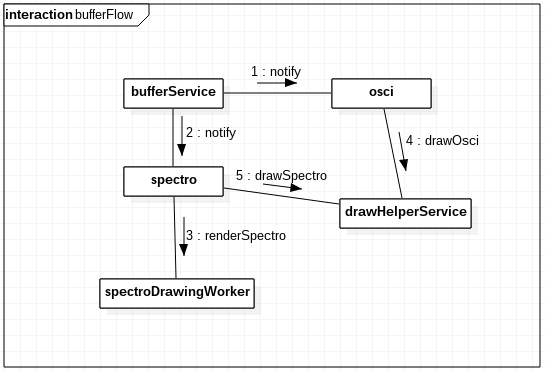
\includegraphics[width=200pt]{figure_1.png}
      \caption{\label{audioFlow} Audio buffer flow}
\end{center}
\end{figure}

This is how the application is working. First, the \textit{Osci} and \textit{Spectro} \textit{Directives} listen to the \textit{BufferService}. It means the when you put an audio buffer in the application, it sends a notification to the \textit{Osci} and \textit{Spectro}. Then, those \textit{directives} use the \textit{drawHelperService} (and the \textit{SpectroDrawingWorker} for the \textit{Spectro}) to display the signal and the spectrogram in the canvas. 

I also add a \textit{Controls Directive} to zoom on the signal, but also to play it. It uses a \textit{appStateService} which contains the start and the end of the signal to be displayed. It also means that the \textit{Osci} and \textit{Spectro Directives} listen to this \textit{Service} too. On \textit{Figure \ref{controlEvent}}, you can figure what \textit{Services} are used.
\begin{figure}[hb]
\begin{center}
   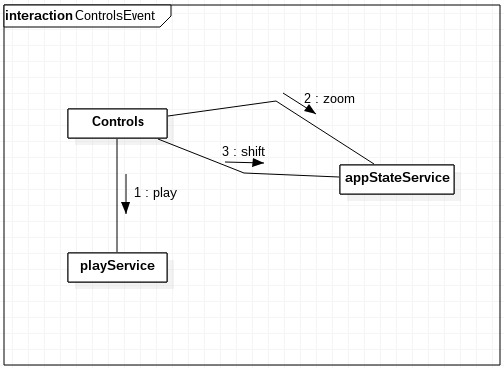
\includegraphics[width=200pt]{figure_2.png}
      \caption{\label{controlEvent} Events from \textit{Controls directive}}
\end{center}
\end{figure}

\section{Proof of concept}
%  - explain what is the goal of the POC and it should be used
%  - explain how you interface the POC with the package (how to install, what piece of code from the
%  POC is related to the package, ...)
%  - the goal of this part is to show how to use the package. Therefore, don't spend too much energy
%  of explaining all the architecture of the POC but focus more on the relation POC/package. However,
%  you have to explain the use case of the POC to make the user understand what is the logic behind

%First talk how to install the package
To install the package, you have two solutions. The first solution is using the package as a regular AngularJS application. You need to have the \texttt{npm} and \texttt{bower} package installated. Then you need to run the following commands in a terminal :
\begin{enumerate}
\item \texttt{npm install grunt}
\item \texttt{bower install}
\item \texttt{npm install}
\end{enumerate}
Then you can run the application using \texttt{grunt serve}. Normally a page should be open on the browser. If no default browser is configured open one brower at the following url: \texttt{http://localhost:9000/}.

The second solution is using the minified code. You need to add the JS scripts in an HTML file. Then you need to add the \texttt{ng-app="EMUInterface"} to the Body tag. Then you need to add a \texttt{<div ng-view=""></div>} to add the views directly in the HTML file. \\

%Then talk how to access the audioBuffer
To use the package, either using minified code or not, you will need to add a new javascript script. You will then need to call the functions in the \textit{bufferService}, using the following javascript code \texttt{angular.element(document.body)  .injector().get('bufferService')}, which gives you an instance of \textit{bufferService}.\\

%Finally talk about how I used that to work with a .WAV file in entry of the application
I implement the package in a small application which takes a .WAV file at the entrance of the application. The script is the following : 
\begin{listing}[1]{1}
var startDraw = function(){
	var bufferService = angular.element(document.body).injector()
	.get('bufferService');
	var browserDetector = angular.element(document.body).injector()
	.get('browserDetector');
	var file = document.getElementById('fileEntry').files[0];
	var reader = new FileReader();
	var res; 

	reader.readAsArrayBuffer(file);

	reader.onloadend = function (evt) {
		if (evt.target.readyState === FileReader.DONE) {
			if (browserDetector.isBrowser.Firefox()) {
				res = evt.target.result;
			} else {
				res = evt.currentTarget.result;
			}
			bufferService.setAudioBufferFromArray(res);
		}
	};
};
\end{listing}

I add a file input in the HTML to call the \texttt{startDraw()} function when the user add a file. This function loads the file and add it in the \textit{BufferService} using the \texttt{setAudioBufferFromArray()} method. Then the application works as explained in the part 2.
\section*{Conclusion}

The next step to improve this project is to add the interface about annotations of a given speech to the package. This should work as the first part, using different functions to render the annotation on a canvas. 

\end{document}